%input macros (i.e. write your own macros file called MacroFile1.tex)
%\newcommand{\PdfPsText}[2]{
  \ifpdf
     #1
  \else
     #2
  \fi
}

\newcommand{\IncludeGraphicsH}[3]{
  \PdfPsText{\includegraphics[height=#2]{#1}}{\includegraphics[bb = #3, height=#2]{#1}}
}

\newcommand{\IncludeGraphicsW}[3]{
  \PdfPsText{\includegraphics[width=#2]{#1}}{\includegraphics[bb = #3, width=#2]{#1}}
}

\newcommand{\InsertFig}[3]{
  \begin{figure}[!htbp]
    \begin{center}
      \leavevmode
      #1
      \caption{#2}
      \label{#3}
    \end{center}
  \end{figure}
}


%%% Local Variables: 
%%% mode: latex
%%% TeX-master: "~/Documents/LaTeX/CUEDThesisPSnPDF/thesis"
%%% End: 


\documentclass[oneside,12pt]{Classes/IITRPRBTP}
\setlength{\arrayrulewidth}{0.5mm}
\setlength{\tabcolsep}{18pt}
\renewcommand{\arraystretch}{1.5}
\usepackage{makecell}
\renewcommand\theadfont{\bfseries}
\usepackage{hyperref}
\usepackage{float}
\usepackage{algorithm}
%\usepackage{algpseudocode}
% \usepackage{arevmath}     % For math symbols
\usepackage[noend]{algpseudocode}

\usepackage{tabularray}
\usepackage{multirow}
\usepackage[table]{xcolor}

%\usepackage[bottom]{footmisc}

\ifpdf
    \pdfinfo { /Title  (IIT Ropar BTech Project Report Classes)
               /Creator (TeX)
               /Producer (pdfTeX)
               /Author (Deepan Maitra 2019csb1044@iitrpr.ac.in)
               /CreationDate (D:20120326000000)  %format D:YYYYMMDDhhmmss
               /ModDate (D:20120326000000)
               /Subject (Writing a BTech Project Report in LaTeX)
               /Keywords (BTP)}
    \pdfcatalog { /PageMode (/UseOutlines)
                  /OpenAction (fitbh)  }
\fi


\title{ Radiogenomic classification of glioblastoma using multimodal 3D MRI}

\renewcommand{\submittedtext}{A Project Report Submitted \\ in Partial Fulfillment of Requirements \\ for the Degree of}
\degree{Bachelor of Technology}
\degreedate{May 2023}

%\vspace{1mm}
\ifpdf
  \author{{by} \\ \href{mailto:2019csb1044@iitrpr.ac.in}{Deepan Maitra (2019CSB1044)} \\ \href{mailto:2019csb1120@iitrpr.ac.in}{Shivani Kumari (2019CSB1120)}}
  \collegeordept{\href{http://www.iitrpr.ac.in}{Department of Computer Science \& Engineering }}
  \university{\href{http://www.iitrpr.ac.in}{Indian Institute of Technology Ropar}}
  \city{{Rupnagar 140001, India}}
% insert below the file name that contains the crest in-place of 'IITRPRlogo'
  \crest{
\includegraphics[width=21mm]{IITRPRlogo}}
%\else
%  \author{Jagpreet Singh}
%  \collegeordept{Department of Computer Science \& Engineering}
%  \university{Indian Institute of Technology Ropar}
% insert below the file name that contains the crest in-place of 'IITRPRlogo'
%  \crest{
\includegraphics[bb = 0 0 292 336, width=30mm]{IITRPRlogo}}
\fi
%
% insert below the file name that contains the crest in-place of 'IITRPRlogo'
% \crest{\IncludeGraphicsW{IITRPRlogo}{40mm}{14 14 73 81}}
%

% turn of those nasty overfull and underfull hboxes
\hbadness=10000
\hfuzz=50pt

% Put all the style files you want in the directory StyleFiles and usepackage like this:
%\usepackage{StyleFiles/watermark}

% Comment out the next line to get single spacing
\onehalfspacing

\begin{document}

%\language{english}

% A page with the abstract on including title and author etc may be
% required to be handed in separately. If this is not so, then comment
% the below 3 lines (between '\begin{abstractseparte}' and 
% 'end{abstractseparate}'), normally like a declaration ... needs some more
% work, mind as environment abstracts creates a new page!
% \begin{abstractseparate}
%   
% Thesis Abstract -----------------------------------------------------


%\begin{abstractslong}    %uncommenting this line, gives a different abstract heading
\begin{abstracts}        %this creates the heading for the abstract page

O6-Methylguanine-DNA methyltransferase (MGMT) promoter methylation status is an important genetic characteristic of glioblastoma and is crucial for it's diagnosis and chemotherapy efficacy. Multimodal MRI imaging techniques can contribute towards monitored automation of invasive surgical approaches. In this body of work, we propose an end-to-end pipeline of tumour segmentation and subsequent radiogenomic classification to classify the given MRI scans into being methylated or non-methylated. We develop a novel Multitask-learning based model (adapted from U-Net) to simultaneously perform segmentation and classification. Further, we utilise the segmentation results to cascade lightweight classification models based on several MRI slice sampling techniques to output the final classification scores. Our resultant pipeline performs well on each of the MRI axes, and several ensembles are tried out to arrive at suitable improvements. Based on 5-fold-cross-validation, we are able to surpass the current Kaggle leaderboard AUCs of the past BraTS RSNA-MICCAI Brain tumour challenge of 2021.


\end{abstracts}
%\end{abstractlongs}


% ----------------------------------------------------------------------


%%% Local Variables: 
%%% mode: latex
%%% TeX-master: "../thesis"
%%% End: 

% \end{abstractseparate}

% Using the watermark package which is in StyleFiles/
% and to remove DRAFT COPY ONLY appearing on the top of all pages comment out below line
%\watermark{DRAFT COPY ONLY}

\renewcommand{\headrulewidth}{0pt}

\maketitle

%set the number of sectioning levels that get number and appear in the contents
\setcounter{secnumdepth}{3}
\setcounter{tocdepth}{3}

\frontmatter % book mode only
\pagenumbering{roman}
%% Thesis Dedictation ---------------------------------------------------

\begin{dedication} %this creates the heading for the dedication page

I would like to dedicate this thesis to my loving parents ...

\end{dedication}

% ----------------------------------------------------------------------

%%% Local Variables: 
%%% mode: latex
%%% TeX-master: "../thesis"
%%% End: 


% Thesis Abstract -----------------------------------------------------


%\begin{abstractslong}    %uncommenting this line, gives a different abstract heading
\begin{abstracts}        %this creates the heading for the abstract page

O6-Methylguanine-DNA methyltransferase (MGMT) promoter methylation status is an important genetic characteristic of glioblastoma and is crucial for it's diagnosis and chemotherapy efficacy. Multimodal MRI imaging techniques can contribute towards monitored automation of invasive surgical approaches. In this body of work, we propose an end-to-end pipeline of tumour segmentation and subsequent radiogenomic classification to classify the given MRI scans into being methylated or non-methylated. We develop a novel Multitask-learning based model (adapted from U-Net) to simultaneously perform segmentation and classification. Further, we utilise the segmentation results to cascade lightweight classification models based on several MRI slice sampling techniques to output the final classification scores. Our resultant pipeline performs well on each of the MRI axes, and several ensembles are tried out to arrive at suitable improvements. Based on 5-fold-cross-validation, we are able to surpass the current Kaggle leaderboard AUCs of the past BraTS RSNA-MICCAI Brain tumour challenge of 2021.


\end{abstracts}
%\end{abstractlongs}


% ----------------------------------------------------------------------


%%% Local Variables: 
%%% mode: latex
%%% TeX-master: "../thesis"
%%% End: 

% Thesis Acknowledgements ------------------------------------------------


%\begin{acknowledgementslong} %uncommenting this line, gives a different acknowledgements heading
\begin{acknowledgements}      %this creates the heading for the acknowlegments


We would like to thank RSNA and the BraTS Kaggle team for their decision to make the competetition dataset publicly available for research purposes. Dr. Deepti R. Bathula has our deepest gratitude, without whom this project would not have taken shape. Finally, we are thankful to the HPC team at IIT Ropar, for their assistance in providing computational GPU resources. 


\end{acknowledgements}
%\end{acknowledgmentslong}

% ------------------------------------------------------------------------

%%% Local Variables: 
%%% mode: latex
%%% TeX-master: "../thesis"
%%% End: 

% Project Owner Code ------------------------------------------------



\begin{honorcode}      %this creates the heading for the certificate

We certify that we have properly cited any material taken from other sources and have obtained permission for any
copyrighted material included in this report. We take full responsibility for any code submitted as part of this 
project and the contents of this report. \\

\vspace*{12mm}

\begin{flushright}
Deepan Maitra (2019CSB1044) \\ \vspace*{5mm} Shivani Kumari (2019CSB1120) \\ 
\end{flushright}

\end{honorcode}


% ------------------------------------------------------------------------

%%% Local Variables: 
%%% mode: latex
%%% TeX-master: "../thesis"
%%% End: 

% Project Certificate ------------------------------------------------



\begin{certificate}      %this creates the heading for the certificate

It is certified that the B. Tech. project \textbf{``Radiogenomic classification of glioblastoma using multimodal 3D MRI"} has been done by \textbf{Deepan Maitra} (2019CSB1044), \textbf{Shivani Kumari}(2019CSB1120) under my supervision. 
This report has been submitted towards partial fulfillment of B. Tech. project requirements. \\

\vspace*{15mm}

\begin{flushright}
\textbf{Dr. Deepti R. Bathula }\\ Associate Professor \\ Project Supervisor \\ Department of Computer Science \& Engineering \\ Indian Institute of Technology Ropar \\ Rupnagar-140001
\end{flushright}


\end{certificate}


% ------------------------------------------------------------------------

%%% Local Variables: 
%%% mode: latex
%%% TeX-master: "../thesis"
%%% End: 


\tableofcontents

\listoffigures
\listoftables
\printnomenclature  %% Print the nomenclature
\addcontentsline{toc}{chapter}{Nomenclature}

\mainmatter % book mode only
%%% Thesis Introduction --------------------------------------------------
\chapter{Introduction}
\ifpdf
    \graphicspath{{Introduction/IntroductionFigs/PNG/}{Introduction/IntroductionFigs/PDF/}{Introduction/IntroductionFigs/}}
\else
    \graphicspath{{Introduction/IntroductionFigs/EPS/}{Introduction/IntroductionFigs/}}
\fi

\nomenclature[zgbm]{$GBM$}{Glioblastoma } 
\nomenclature[zmri]{$MRI$}{Magnetic Resonance Imaging } 
\nomenclature[zmgmt]{$MGMT$}{O6-Methylguanine-DNA methyltransferase } 
\nomenclature[zmtl]{$MTL$}{Multi Task Learning } 
\nomenclature[ztmz]{$TMZ$}{Temozolomide } 
\nomenclature[zauc]{$AUC$}{Area Under Curve } 
\nomenclature[gp]{$\pi$}{ $\simeq 3.14\ldots$}  
\nomenclature[rj]{$j$}{superscript index} 
\nomenclature[s0]{$0$}{subscript index}

Glioblastoma multiforme (GBM) is the most probable category of brain tumour that affects adults. Over 45\% of primary central nervous system tumours are accounted by GBM, and the patient survival rate is around 5.1\% for a five-year period (as documented in \cite{GBM_survival}). 

%\cite{Sim90}


\section {Motivation}
O6-methylguanine-DNA methyltransferase (MGMT) promoter is a significant  molecular biomarker of glioblasoma that has relevance in cancer theurapeutics. MGMT is one of the DNA repair enzymes and the methylation status of its promoter in newly diagnosed GBM tumour has been identified as a predictor of chemotherapy response (\cite{GBM_chemo}).  The survival benefit governed by the MGMT gene methylation status during temozolomide (TMZ) treatment was observed by \cite{GBM_TMZ}. Further work has asserted that for patients who received chemotherapy through temozolomide, the methylation status of the MGMT promoter gene improved median survival compared with patients who had unmethylated gliomas. Thus, MGMT methylation status as reported in 30-60\% of glioblastomas can enhance the response to TMZ (as recorded in \cite{GBM_TMZ_2}).
\vspace*{3mm} 

Currently, surgical specimens based genetic lab testing is the standard to assess the MGMT methylation status of GBM. In this method, a large tissue sample is required, which is tested by polymerase chain reaction (PCR) to judge the methylation status(\cite{biopsy_1}). The major limitations of this invasive methodology are the possibility of incomplete biopsy samples due to tumour spatial heterogeneity and the high cost involved in tissue sampling (\cite{biopsy_2}). It can lead to neurological injury and nerve damage during the operative procedure. Therefore, there is a neccessity to find non-invasive methods based on brain imaging, which can successfully lead to an effective prediction of the methylation status of glioblastoma.

\section{MRI Imaging}
Magnetic Resonance Imaging (MRI) is a popular diagnostic tool in detection and treatment of GBM tumours (\cite{MRI_1}) The monitired, coordinated use of multiple, mutually informative imaging probes to understand brain structure and function has given raise to multimodal MRI imaging techniques, that has shown greater visibility of gliomas. 

\vspace*{3mm} 
In recent studies in radiogenomics, it has been shown that quantitative and qualitative features extracted from medical images can have a direct correlation with the genetic traits of the tissues. In this regard, radiogenomic data can be directly utilized to analyse the MGMT methylation status of the GBM tumour. (\cite{MRI_2} and \cite{MRI_3}). However, feature extraction from MRI images can be a cumbersome process as it involves a manual differentiation of the glioma tumour region from rest of the grey matter. Information analytics of the extracted feature is also prone to disagreement between the observers responsible for the tumour segmentation (\cite{MRI_4} and \cite{MRI_5})

\section{Deep learning approaches}

With the boom in deep learning techniques in medical imagings, several researchers have taken up the problem of GBM tumour diagnosis. Deep learning can enable automatic extraction of features based on the given loss function optimization for the particular use case (\cite{DL_1}). 

\vspace*{3mm} 
Convolutional Neural Networks (CNNs) make use of the convolution operation in images, and has been effective in image analysis. (\cite{DL_2}, \cite{DL_3}, \cite{DL_4}). As compared to traditional methods with hand-crafted features, deep learning methods has advantages of being robust to image distortions like changes in shape, orientation and involves a lower computational cost. The neural network architecture has the capacity to `learn' weights on its own when supplied with a considerably large training set, and this predictive ability has been widely beneficial. 

\vspace*{3mm} 
Although multiple radiomic approaches have used deep learning to predict the MGMT gene methylation, the clinical viability of the prediction and its reliability when compared to surgical diagnosis by physicians is a matter of open research. \cite{DL_5} performed texture analysis on MR images to predict MGMT promoter methylation status, whereas \cite{DL_6} used combined texture features along with supervised classification schemes as imaging biomarkers. 

\vspace*{3mm} 
There remains a scope for investigation of a complete end-to-end pipeline that can do automatic tumour detection, tumour region segmentation and subsequent MGMT methylation classification, with minimum user intervention. Since the MRI scans are often supplied as 3D volumes, efficient 2D sampling should be a crucial element of the model pipeline. We thereby try to come up with such an architecture that can achieve the discussed use cases.  








%%% ----------------------------------------------------------------------


%%% Local Variables: 
%%% mode: latex
%%% TeX-master: "../thesis"
%%% End: 

% \pagebreak[4]
% \hspace*{1cm}
% \pagebreak[4]
% \hspace*{1cm}
% \pagebreak[4]



\chapter{BraTS 2021 challenge and Kaggle leaderboard}
\ifpdf
    \graphicspath{{Kaggle/Chapter1Figs/PNG/}{Kaggle/Chapter1Figs/PDF/}{Kaggle/Chapter1Figs/}}
\else
    \graphicspath{{Kaggle/Chapter1Figs/EPS/}{Kaggle/Chapter1Figs/}}
\fi

% \begin{eqnarray}
% CIF: \hspace*{5mm}F_0^j(a) &=& \frac{1}{2\pi \iota} \oint_{\gamma} \frac{F_0^j(z)}{z - a} dz
% \end{eqnarray}



                              % first letter Z is for Acronyms 
% \nomenclature[aF]{$F$}{complex function}                                                   % first letter A is for Roman symbols
                                           % first letter G is for Greek Symbols
% \nomenclature[gi]{$\iota$}{unit imaginary number $\sqrt{-1}$}                      % first letter G is for Greek Symbols
% \nomenclature[gg]{$\gamma$}{a simply closed curve on a complex plane}  % first letter G is for Greek Symbols
% \nomenclature[xi]{$\oint_\gamma$}{integration around a curve $\gamma$} % first letter X is for Other Symbols

% first letter R is for superscripts                                                        % first letter S is for subscripts




The Radiological Society of North America (RSNA) teamed up with the Medical Image Computing and Computer Assisted Intervention Society (MICCAI) to improve the treatment planning for patients with glioblastoma. The RSNA-ASNR-MICCAI BraTS 2021
challenge (\cite{Brats}) targetted the evaluation of ML algorithms assessing
the tumour region segmentation, as well as the underlying tumor’s molecular characterization, in pre-operative baseline MRI imaging data. Specifically, the two tasks that BraTS 2021 focuses on are: a) the segmentation of the histologically distinct brain tumor sub-
regions, and b) the classification of the tumor’s O[6]-methylguanine-DNA
methyltransferase (MGMT) promoter methylation status. 

\vspace*{3mm} 
 The part 2 of the competition which involves predicting the MGMT methylation status of the given patient MRI smaples was hosted on Kaggle\footnote{\href{https://www.kaggle.com/competitions/rsna-miccai-brain-tumor-radiogenomic-classification}{https://www.kaggle.com/competitions/rsna-miccai-brain-tumor-radiogenomic-classification}}. Kaggle is an online community of data scientists and machine learning practitioners.
\vspace*{8mm}

\hypersetup{ colorlinks=true,
    linkcolor=black,
    filecolor=magenta,      
    urlcolor=blue}

\section{Current Kaggle leaderboard}
% \begin{figure}[!htbp]
%   \begin{center}
%     \leavevmode
%     \ifpdf
%       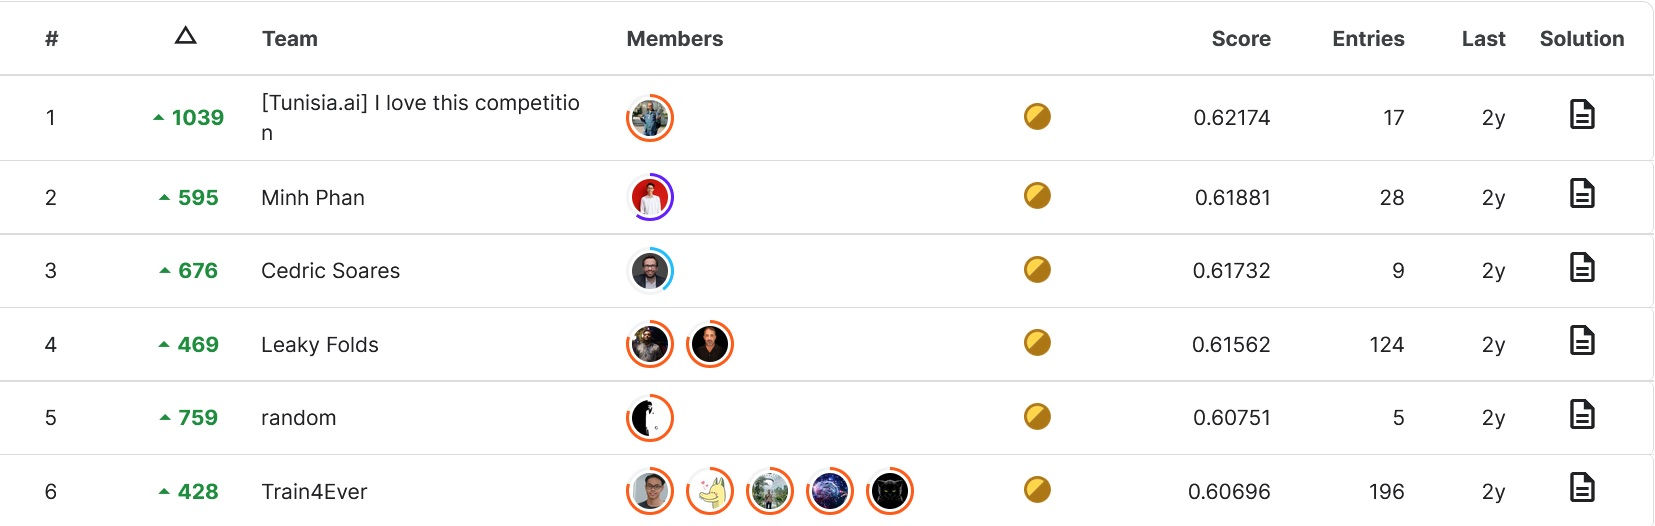
\includegraphics[height=2in]{Kaggle_leaderboard}
%     \else
%       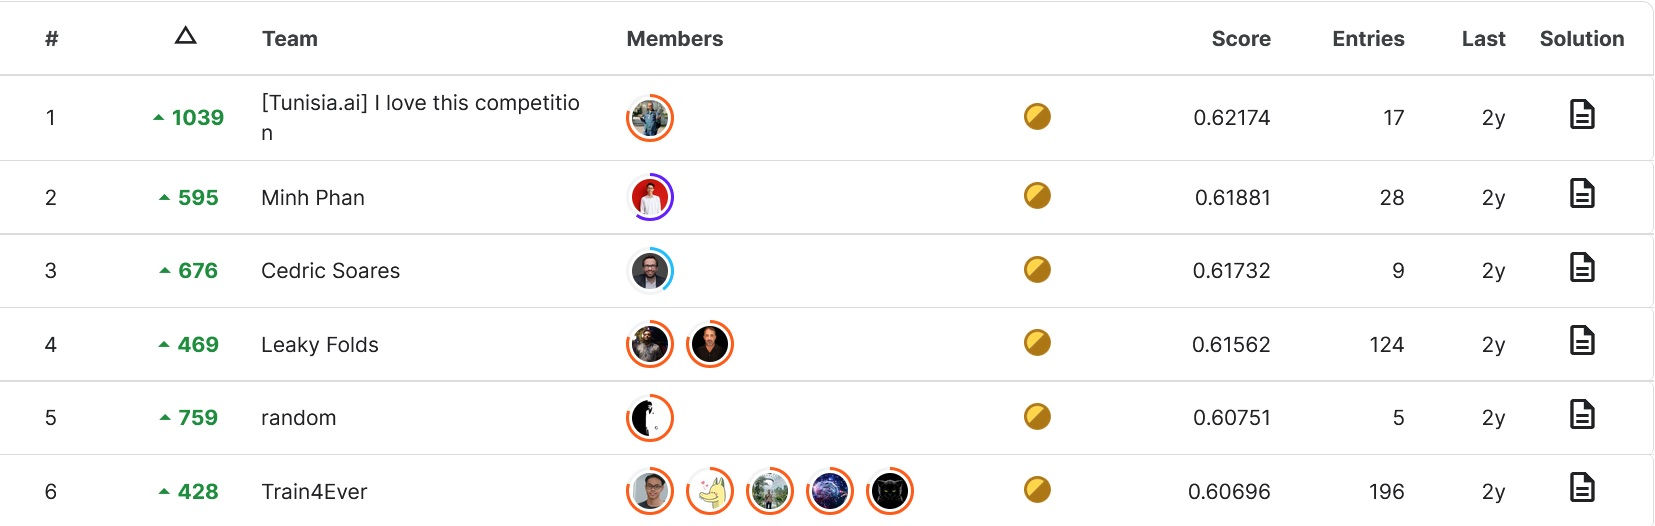
\includegraphics[bb = 92 86 545 742, height=6in]{Kaggle_leaderboard}
%     \fi
%     \caption{Kaggle leaderboard Top 6 teams}
%     \label{FigKaggleLeaderboard}
%   \end{center}
% \end{figure}
The Kaggle 2021 competition saw the participation of 1555 teams. The following table summarizes the model architectures and scores of the top six teams of the currently featuring \href{https://www.kaggle.com/competitions/rsna-miccai-brain-tumor-radiogenomic-classification/leaderboard}{leaderboard}. 

\vspace*{6mm}
\begin{table}[h!]
\centering
\begin{tabular}{ p{2cm} p{5.5cm} p{4cm}  }
 \hline
 \multicolumn{3}{c}{\thead{Current BraTS 2021 leaderboard}} \\
 [0.8ex]
 \hline
  \thead{Rank} & \thead{Model used} & \thead{AUC performance} \\  [0.8ex]
 \hline
 1   & 3D CNN + ResNet    & 0.621 \\  [0.8ex]
 2 &   EfficientNet + LSTM  & 0.618   \\  [0.8ex]
 3 & 4 parallel EfficientNet & 0.617  \\  [0.8ex]
 4 & YOLO (2D) + 3D CNN & 0.615 \\  [0.8ex]
 5 &   EfficientNet  & 0.607 \\  [0.8ex]
 6 & UNet + LSTM  & 0.606 \\  [0.8ex]
 \hline
\end{tabular}
\caption{Kaggle leaderboard top 6 teams}
\label{table:1}
\end{table}

\vspace*{6mm}

The \textbf{Rank 1} team uses a combination of 3D CNNs and a popular ResNet architecture to stack the 2D scans around an appropriately chosen 2D middle slice (from given DCM files) and then pass the 3D volume for classification. 3D CNNs are computationally exhaustive and require a heavy GPU for the larger convolutional load. The \textbf{Rank 2} team uses a complex sampling stretegy to introduce sequentiality into the data. They sample 10 scans from all patients (uniform temporal subsampling) across the 4 MRI modalities (T1cE, T2cE, T1wCE, Flair) to get 4-slice stacks which were fed into an LSTM network. 

\vspace*{3mm}

The \textbf{Rank 3} team uses 4 EfficientNet networks parallely for each of the 4 given modalities. The networks are simulatenously trained during the training phase, but in the testing phase, for each modality, predictions are obtained on a slice-by-slice basis and the most confident prediction probability is selected. Finally on the patient level, the average across 4 modality is obtained. The \textbf{Rank 4} team uses YOLO models on the 2D slices to detect the slices which have the best tumour visibility and then feed them into pre-trained classification networks. The \textbf{Rank 5} team sampled 10 images from each modality (patient level), took pixel intensity average of the 10 images to obtain one single image per modality, then stacked them together to get 4-slice-stacks. It was then fed to an EfficientNet model. Lastly, the \textbf{Rank 6} team sampled 2D slices from segmentation masks (with high tumour visibility) to get 2 masks (Tumour core, Enhancing tumour). The 2D slice was stacked with 2 kinds of mask to get 3-slice input, which was then fed to an LSTM network in chunks. 



\vspace*{6mm}

\hypersetup{ colorlinks=true,
    linkcolor=black,
    filecolor=magenta,      
    urlcolor=black}

\section{Observations and Scope}

The leaderboard test dataset AUCs saturate at around 0.61.
Observing the leaderboard approaches, it can be sensed that less focus is being given to localize the tumour voxel and then feed the Region-of-interest into a suitable classification network. Hence, the utility of an efficient Tumour segmentation task becomes apparent. Localization of the tumour region can be done in 2D slice basis or by taking into account the whole 3D volume. In this report, we highlight our investigations in this direction.  
\vspace{3mm}

It is to be noted that the tumour segmentation and Multi-task model based experiments was conducted in the Autumn semester (Sem 1 2022-23) while the volumetric projections and cropped-cascaded model tests were conducted in the Spring semester (Sem 2 2022-23). The source code, implementations, models can be found in the GitHub\footnote{\href{https://github.com/Deepan2486/Radiogenomic-classification-glioblastoma-multimodal-3D-MRI}{https://github.com/Deepan2486/Radiogenomic-classification-glioblastoma-multimodal-3D-MRI}} repository.
% \cite{texbook}

% \subsection{sub first paragraph}
% ... and some more ...



% above code has been macro-fied in Classes/MacroFile.tex file
%\InsertFig{\IncludeGraphicsH{aflow}{6in}{92 86 545 742}}{Airfoil Picture}{FigAir}

% So as we have now labelled it we can reference it, like so (\ref{FigKaggleLeaderboard}) and it
% is on Page \pageref{FigKaggleLeaderboard}. And as we can see, it is a very nice picture and we
% can talk about it all we want and when we are tired we can move on to the next
% chapter ...

\ifpdf
  \pdfbookmark[2]{bookmark text is here}{And this is what I want bookmarked}
\fi
% ------------------------------------------------------------------------


%%% Local Variables: 
%%% mode: latex
%%% TeX-master: "../thesis"
%%% End: 

\chapter{Dataset and Experimental set-up}
\ifpdf
    \graphicspath{{Experimental/Chapter2Figs/PNG/}{Experimental/Chapter2Figs/PDF/}{Experimental/Chapter2Figs/}}
\else
    \graphicspath{{Experimental/Chapter2Figs/EPS/}{Experimental/Chapter2Figs/}}
\fi

\section{Dataset}


The Brain Tumour Segmentation Challenge (BraTS) dataset describes a collection of brain tumor MRI scans acquired from multiple institutions under standard clinical conditions, but with different imaging protocols. The data inclusion criteria comprised pathologically confirmed carcinoma diagnosis and
available MGMT promoter gene methylation status (\cite{Brats})

\subsection{Dataset description}

\vspace*{3mm} 
The BraTS 2021 task was classified into two phases:
\begin{enumerate}
    \item \textbf{Tumour region segmentation (Phase 1)}: This phase was hosted on the \href{https://www.synapse.org/#!Synapse:syn27046444/wiki/616571}{Synapse} platform. The mpMRI scans describe a) native (T1) and b) post-contrast T1-weighted, c) T2-weighted (T2), and d) T2 Fluid Attenuated Inversion Recovery (T2-FLAIR) volumes. After standard pre-processing, the DICOM data files was converted to NIfTI file format (\cite{seg_1}). Co-registration to the same anatomical template (SRI24) was performed (as in \cite{seg_2}) and the scans were resampled to a uniform isotropic resolution (1mm3), and finally skull-stripped. To construct the training set, all imaging volumes were segmented using the STAPLE fusion (\cite{seg_3}) and then manually annotated by radiological experts. 

    \item \textbf{Radiogenomic classification (Phase 2)} : This phase was hosted on \href{https://www.kaggle.com/competitions/rsna-miccai-brain-tumor-radiogenomic-classification/overview}{Kaggle}. The annotated NIfTI files were again converted into a series of DICOM scans (in the patient space) using \href{https://cbica.github.io/CaPTk/}{CaPTk’s} NIfTI to DICOM conversion engine. This process is repeated across the 4 modalities. The Pyromark CpG MGMT kit detected the average level of methylation on CpG 74–81 sites located in the MGMT gene. The percent methylation above 10\% was interpreted as positive. A sample below 10\% methylation was interpreted as negative
\end{enumerate}

\subsection{MRI modalities}
\vspace*{5mm} 

MRI is based on the magnetization properties of atomic nuclei. By chnaging the sequence of Radio Frequency pulses applied, different types of images are created. Repetition Time (TR) is defined as the time  duration between successive pulse sequences applied to a partiucular slice. Time to Echo (TE) is the time duration between the delivery of the RF pulse and the receipt of the echo signal. The most common MRI sequences are T1-weighted and T2-weighted scans. \textbf{T1-weighted} images are produced by using short TE and TR times. \textbf{T2-weighted} images are produced by using longer TE and TR times. In general, T1- and T2-weighted images can be easily differentiated by looking the Cerebro-spinal-fluid (CSF), which is dark on T1-weighted imaging and bright on T2-weighted imaging. A third modality is \textbf{Fluid Attenuated Inversion Recovery (Flair)}. The Flair sequence is similar to a T2-weighted image except that the TE and TR times are very long. T1-weighted imaging can also be performed while infusing a non-toxic paramagnetic contrast enhancement agent Gadolinium (Gad). When injected, Gad changes signal intensities. It is termed as \textbf{T1-contrast-enhanced} images and are especially useful in looking at vascular structures. The visibility of brain structures in the modalities can be described as:
\begin{table}[H]
\centering
\begin{tabular}{ p{2.8cm} p{2cm} p{2.2cm} p{2.2cm} }
 % \hline
 % \multicolumn{3}{c}{\thead{Current BraTS 2021 leaderboard}} \\
 % [0.8ex]
  \hline
  \thead{ } & \thead{T1w} & \thead{T2w} & \thead{Flair} \\ 
 \hline
 \textbf{CSF}   & Dark    & Bright & Dark \\  [0.8ex]
 \textbf{White matter}  & Light    & Dark grey & Dark grey \\  [0.8ex]
 \textbf{Cortex}   & Grey    & Light Grey & Light Grey \\  [0.8ex]
 \hline
\end{tabular}
\caption{Brain tissue visibility in MRI}
\label{table:2}
\end{table}

% \vspace*{4mm}
The MRI scan modalities are depicted below, represented across the 3 axis (\textbf{axial, coronal and saggital}). 
%\vspace*{4mm}

\begin{figure}[H]
  \begin{center}
    \leavevmode
    \ifpdf
      \includegraphics[height=3.6in, width=5.7in]{Experimental/Chapter2Figs/modality_3_axis.jpeg}
    \else
      \includegraphics[bb = 92 86 545 742, height=6in]{modality_3_axis}
    \fi
    \caption{Modalities across 3 axis. \textbf{A1-A3} depict T1-weighted images, \textbf{B1-B3} as T2-weighted, \textbf{C1-C3} as T1-contrast-enhanced and \textbf{D1-D3} as Flair. The first row is the \textbf{axial} direction, then \textbf{coronal} and \textbf{saggital} showing the various positions of the tumour}
    \label{modality_3_axis}
  \end{center}
\end{figure}

% \vspace*{4mm}

As observed, the Flair scan images gives the best tumour voxel visibility by illuminating the tumour tissue with pixel intensity very different from the surrounding region. The T1cE scans outline the tumour regions and depict the vascularity. The T1 and T2 scans are not representative enough of the tumour location, as assessed by monitoring multiple cases from the dataset.

\subsection{Number of samples}
\vspace*{3mm}
The patients were uniquely labelled with a number called the BraTS21-ID. There were 595 datapoints provided as segmentation masks and 585 classification ground-truth labels were given. In all, \textbf{573 unique patient IDs} could be utilised for experimentation purposes. Out of these, \textbf{298} were labelled as methylated and \textbf{275} were unmethylated. So, class imbalance was minimal.
\vspace*{3mm}

Each of the unique BraTS21-ID had five NIfTI files (correspodning to T1-weighted, T2-weighted, T1-contrast-enhanced, Flair and the multiclass segmentation mask) along with the classification true labels. All the NIfTI files were voulmetric with dimensions \textbf{(240,240,155)} which meant that 2D slices of dimensions \textbf{240 x 240} were stacked on top of one another to form a height of 155 slices. The methylation status labels were 0 or 1 (binary classification)
\vspace*{3mm}

In experimentations without a cross-validation step, 20\% of the datapoints were reserved for testing and the rest 80\% for training purposes. Further, during training the validation split was 0.2. So, among 573 samples, \textbf{458} were used for training, \textbf{115} for testing (within training, 91 datapoints were used internally for validation). 
\vspace*{3mm}

In experiments where we used 5-fold-cross validation, the entire dataset was divided into 5 chunks of \{114,114,115,115,115\} datapoints. During each fold, one of the sets was used as a test set and a stratfied combination of the other 4 as the training set. 



\subsection{Tumour segmentation regions}
\vspace*{1mm} 
The tumour segmentation part of the task involves dividing the localized tumour regions into pixel categories of \{0,1,2,3\} based on the kind of tumour tissue. The classes are as follows:

\begin{enumerate}
    \item \textbf{Label 0} : The background region
    \item \textbf{Label 1} : Necrotic Tumour Core NCR
    \item \textbf{Label 2} : peritumoral edematous invaded tissue (ED)
    \item \textbf{Label 3} : Gd enhancing tumour (ET)
    
\end{enumerate}

ET is the enhancing portion of the tumor, described by areas with faint enhancement on T1Gd (T1CE) MRI. NCR is the necrotic core of the tumor, the appearance of which is intense on T1cE MRI. ED is the peritumoral infiltrated tissue, defined by the abnormal
hyperintense envelope on the T2-weighted and FLAIR volumes. They include the infiltrative non enhancing tumor. 
\vspace*{3mm}

\begin{figure}[H]
  \begin{center}
    \leavevmode
    \ifpdf
      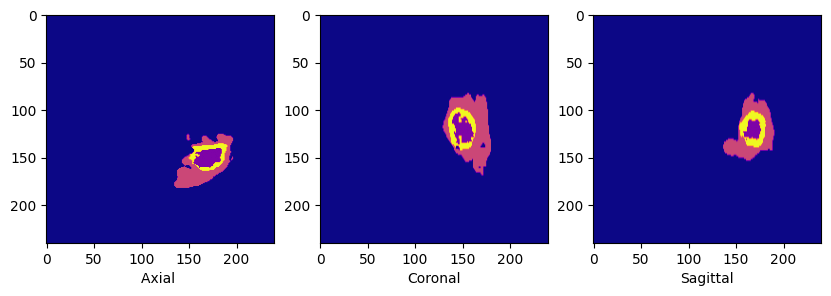
\includegraphics[height=2in]{Experimental/Chapter2Figs/tumour_regions.jpg}
    \else
      \includegraphics[bb = 92 86 545 742, height=6in]{tumour_region}
    \fi
    \caption{Tumour regions (in the axial, coronal, saggital directions). The different colours depict the multiclass pixel labels}
    \label{tumour_region}
  \end{center}
\end{figure}
As can be seen, the tumour regions are distinctly prominent in all the 3 directional axes. These mask categories are independent of the MRI modality. They show the ground-truth labels of the pixels that depict the tumour tissue. 

\subsection{Methylated and Non-methylated tumours}
%\vspace*{1mm}
According to the discussed background of the problem, the methylation status of the MGMT gene can be correlated with biomarkers in the MRI scan. The methylation status can be informally judged by looking at the distribution of the tumour pixel categories, and in the way the tumour region is spread out. 

%\vspace*{2mm}


\begin{figure}[H]
  \begin{center}
    \leavevmode
    \ifpdf
      \includegraphics[height=2.9in]{Experimental/Chapter2Figs/methylated_unmethylated.jpg}
    \else
      \includegraphics[bb = 92 86 545 742, height=6in]{methylated_unmethylated}
    \fi
    \caption{(A) Unmethylated tumours and (B) Methylated tumours}
    \label{methylated_unmethylated}
  \end{center}
\end{figure}

The unmethylated tumour exmaples in (A) have a less-defined tumour core region, and although the invaded tissue extent is large, the necrosis of the core is subdued. Whereas in methylated samples (B), the tumour core is starkly prominent and the tumour growth is visible from inside-out.
\vspace*{2mm}

The methylation classification of the tumour is challenging because the tissue biomarker of the underlying genomic characteristic is not directly inferrable. In the methylation ground-truth labels provided as training data, a 10\% benchmark across the gene sites was considered for the binary classification. Since the MRI scans can have varying levels of carninoma and the MGMT methylation percentage can vary, therefore there remains some sort of ambiguity in the visible differences. 

\section{Model architectures}

Various model architectures were experimented for the segmentation and classification tasks. All the models that were based on 2D Convolutional Neural Networks (CNN) and the input data had multiple channels based on the requirement.

\subsection{UNet 2D }
\vspace*{2mm}
U-Net was introduced by \cite{Unet} for highly accurate biomedical semantic image segmentation. It gained popularity because it required less number of training samples. 
\vspace*{2mm}

UNet is based upon the encoder-decoder model of deep CNN archictecture and incorporates an encoder block, skip connections and a decoder block. It combines feature extraction and feature localization strategies. 

\begin{enumerate}
    \item \textbf{Encoder block:} Encoder captures the most relevant information in the input image into a lower-dimesnional space, by extracting the most definitive features. It uses a series of convolution, pooling and fully-connected layers to arrive at a compact representation. 
    \item \textbf{Decoder Block}: Decoder block is the exact opposite of the encoder operation. By using the compact feature representation, it reconstructs the image by using deconvolutional and upsampling operations which increase the image dimensionality.
    \item \textbf{Skip connections}: This step is crucial for preserving the locational or spatial information of the image. In U-Net, skip connections are used to pass information from earlier convolutional layers to the deconvolution layers. What is passed is the location of the feature extracted by convolutional layers. This is done by concatenating the last layer in the convolutional block with the first layer of the opposite deconvolutional block.
\end{enumerate}

The UNet architecture is symmetrical and the dimensions of the opposite layers/blocks will be the same. If we input a (X,Y) dimensional 2D image which is to be semantically segmented to 4 classes, then the output image will be (X,Y,4) in the categorical data format.

\subsection{Multi-task-learning (MTL) model}
\vspace*{2mm}
A novel Multi-task-learning model was developed from an UNet adaptation. Multi-task-learning models refers to networks which are optimized for more than one task, and they simultaneously train the network parameters for all the tasks. By sharing representations between the related tasks, it avoids overfitting and enables the model to learn better.
\vspace*{2mm}

In our problem statement, the \textbf{segmentation} and \textbf{classification} tasks are related to one another and can be learnt jointly. We employ \textbf{Hard parameter sharing} in which there are task-specific individual layers and shared layers. Shared layers have to learn parameters that fit both the given tasks. The model back-propagates along both the individual and the shared layers.

\begin{figure}[H]
  \begin{center}
    \leavevmode
    \ifpdf
      \includegraphics[height=2.1in]{Experimental/Chapter2Figs/MTL_shared.png}
    \else
      \includegraphics[bb = 92 86 545 742, height=6in]{MTL_shared}
    \fi
    \caption{A general MTL model showing shared and task-specific layers}
    \label{MTL_shared}
  \end{center}
\end{figure}

The semantic segmentation model of UNet was adapted into an MTL model by adding the \textbf{classification branch}. The classification branch utilizes the compact feature representations from the lowest 3 blocks of the UNet (one from encoder, one from decoder and the bridge layer). Since these 3 blocks have outputs of different dimensionality, we use a \textbf{Global Average Pooling (GAP)} layer after each, which scales down the input dimensions of \textbf{(X, Y, Z)} to \textbf{(1, 1, Z)} by doing a average operation. The reduced image features are then joined by a concatenation layer which is passed to a Fully-connected layer (with Softmax activation function) to get the final binary classification. For any test image, a two-tuple output is given by the model. The 1st output is the segmentation mask, and the 2nd output is the probability of the classification label (methylated/ unmethylated). 
\begin{center}
    $L_{joint} = \lambda L_{cls} + (1-\lambda) L_{seg}$
\end{center}
%\vspace*{1mm}
The loss function of an MTL model is jointly given by the loss of the classification $L_{cls}$ and the loss of segmentation $L_{seg}$, weighted by a parameter $\lambda$. By changing the value of $\lambda$ we can give more weightage to either of the tasks.
\vspace*{4mm}

\begin{figure}[H]
  \begin{center}
    \leavevmode
    \ifpdf
      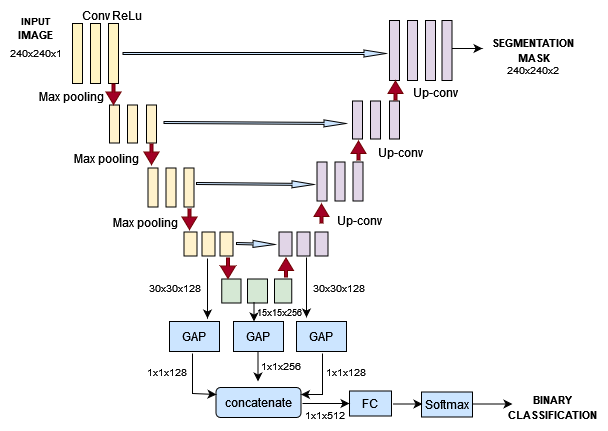
\includegraphics[height=4in]{Experimental/Chapter2Figs/MTL.png}
    \else
      \includegraphics[bb = 92 86 545 742, height=6in]{MTL_fig}
    \fi
    \caption{Our U-Net adapted MTL model}
    \label{MTL_fig}
  \end{center}
\end{figure}


\subsection{ResNet18 and ResNet34}
\vspace*{3mm}
A new category of deep networks called \textbf{Residual networks (ResNet)} was introduced in \cite{resnet}. The layers are reformulated to learn residual functions with reference to the layer inputs, instead of learning unreferenced functions. These ResNets are easier to optimize, and can gain accuracy from considerably increased depth. By using \textbf{'skip connections'} periodically in the model architecture,  activations of a layer are connected to further layers by skipping some layers in between, thus forming a \textbf{'Residual Block'}. Identity shortcut connections add neither extra parameter nor computational complexity. The entire network can still be trained with back propagation.

%\vspace*{1mm}

\begin{figure}[H]
  \begin{center}
    \leavevmode
    \ifpdf
      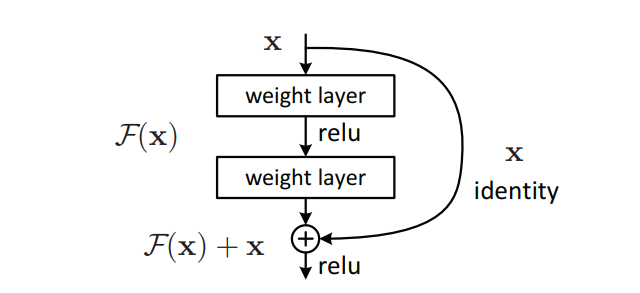
\includegraphics[height=2in]{Experimental/Chapter2Figs/residual_block.PNG}
    \else
      \includegraphics[bb = 92 86 545 742, height=2.5in]{Residual}
    \fi
    \caption{A simple Residual Block (cited from \cite{resnet})}
    \label{Residual}
  \end{center}
\end{figure}

ResNet uses a network architecture inspired by VGG-19 (\cite{vcg19}) in which shortcut connections are added. On the ImageNet dataset,  the authors of the paper uses a 152-layers ResNet, which is 8 times more deep than VGG19 but still have less parameters. In general, \textbf{ResNet18} and \textbf{ResNet34} are used for smaller classification tasks which are 18 layers and 34 layers deep respectively.


\subsection{EfficientNet}
\vspace*{3mm}
A new family of models called EfficientNet was introduced in \cite{effnet}. The EfficientNet architecture uniformly scales all dimensions of depth/width/resolution using a compound coefficient (\textbf{model scaling}). The EfficientNet scaling method uniformly scales network width, depth, and resolution with a set of fixed scaling coefficients, rather than using arbitrary scaling factors.
\vspace*{3mm}

The baseline model \textbf{EfficientNet B0} is based on the inverted bottleneck residual blocks that was demonstrated in MnasNet (\cite{mnasnet}), in addition to the squeeze-and-excitation blocks. The building block of this architecture is the mobile inverted bottleneck MBConv  (inverted residual block) with an additional Squeeze-and-Excitation block. Using compound scaling, \textbf{ EfficientNet B1} to \textbf{EfficientNet B7} are developed, where the number of model parameters increase exponentially, but give higher accuracy. 


% ------------------------------------------------------------------------

%%% Local Variables: 
%%% mode: latex
%%% TeX-master: "../thesis"
%%% End: 

\chapter{Methodology}
\ifpdf
    \graphicspath{{Chapter3/Chapter3Figs/PNG/}{Chapter3/Chapter3Figs/PDF/}{Chapter3/Chapter3Figs/}}
\else
    \graphicspath{{Chapter3/Chapter3Figs/EPS/}{Chapter3/Chapter3Figs/}}
\fi

\section{Multi-Task-Learning (MTL) model}\label{MTL}
\vspace*{3mm}
As depicted in Figure \ref{MTL_fig}, the segmentation-classification MTL model performs multiclass segmentation to get the detected tumour region from the MRI, and also gives the prediction probability of the binary classification of the glioblastoma being methylated/unmethylated. (Results are summarized in section \ref{MTL_results})
\vspace*{3mm}

We only need an accurate tumour localization in the segmentation step, so we change the tumour masks from being 4-class of labels \{0,1,2,3\} to being a binary mask of labels \{0,1\}. This is done by simply equating the non-zero pixel labels to 1. The below figure shows some examples:
\vspace*{4mm}
\begin{figure}[H]
  \begin{center}
    \leavevmode
    \ifpdf
      \includegraphics[height=1.5in]{Methodology/Chapter3Figs/binary_mask.png}
    \else
      \includegraphics[bb = 92 86 545 742, height=6in]{binary_mask}
    \fi
    \caption{Tumour Binary masks}
    \label{binary_mask}
  \end{center}
\end{figure}

\begin{center}
    $L_{joint} =\displaystyle \lambda L_{cls} + (1-\lambda) L_{seg}$
\end{center}
%\vspace*{1mm}
The loss function of an MTL model is jointly given by the loss of the classification $L_{cls}$ and the loss of segmentation $L_{seg}$, weighted by a parameter $\lambda$. The variable $\lambda$ ranges from [0,1] and is used as a hyperparameter. 
\vspace*{3mm}

For the binary classification task, we use \textbf{Focal Loss} as the loss function. For segmentation, we experimented with both \textbf{Binary Cross Entropy} and \textbf{Dice Loss}. 
\vspace*{3mm}
\begin{center}
    $ BCE Loss= -\displaystyle\frac{1}{N}\displaystyle\sum\limits_{i=1}^N  (y_i\log(p_i) + (1 - y_i)\log(1 - p_i))$
    \vspace*{3mm}
    
   $Focal Loss = \displaystyle\sum\limits_{i=1}^N (i-p_i)^{\gamma}\log_(p_i)$
\vspace*{3mm}

$Dice Loss = 1 - \displaystyle\frac{1 + 2*P_s*Y_s}{1 + P_s + Y_s}$
   
    
\end{center}
\vspace*{3mm}

In Focal Loss, the \textbf{Focusing Parameter} $\gamma$ controls the class imbalance in the classification labels and also reduces the influence of easy examples on the loss function, resulting in more attention being paid to hard examples (\textbf{Down Weighting}). N is the total number of classes (here 2), $y_i$ is the true label of the classification and $p_i$ is the prediction probability.
\vspace*{3mm}

In BCE Loss (used for segmentation), $y_i$ represents the true tumour label mask, and $p_i$ represents the predicted tumour label mask. For the segmentation task, the imbalance between foreground and background may cause segmentation bias. To account for this problem, a segmentation loss based on the Dice coefficient (Dice Loss) is utilized to emphasize shape similarity between actual and predicted segmentation maps. For Dice Loss, $Y_s$ is the actual tumour mask whereas $P_s$ is the predicted tumour mask. 
\vspace*{3mm}

Two approaches were taken for the MTL experimentation. Since the model is trained for 2D images, fitting in the entire 3D volume is not feasible. We therefore employ 2 sampling methods:

\begin{enumerate}
    \item \textbf{Middle slice}: We use the middle slice (slice=70) from each NIfTI scan, and then pass this 2D image into the network. The mask for training is also sampled by taking slice=70 from the corresponding true mask.
    \item \textbf{10 slices from each volume}: In order to introduce variability in the dataset, we sample 10 slices from the entire 155 slices. The samples are taken by eliminating the upper and lower 20\% of the slices (since they hardly have any relevant tumour information). Iteratively we save one slice after another by spacing out 2 slices in between. This way, the dataset slices increases 10-fold. During the sampling, a check is employed to ensure that the slice has the requisite tumour visibility. If not the case, then we move to a new slice. This method trains the MTL model towards predicting unseen tumours of varying shapes and structure.
\end{enumerate}


\section{Volumetric Projections}\label{volumetric}
\vspace*{3mm}

Since the dataset dimensions are (240,240,155) where 155 is the number of slices in each scan, there is a need to capture the entire 3D spatial information into a 2D dimension. We therefore utilize various projection approaches to experiment. 
\begin{figure}[H]
  \begin{center}
    \leavevmode
    \ifpdf
      \includegraphics[height=2in]{Methodology/Chapter3Figs/proj.png}
    \else
      \includegraphics[bb = 92 86 545 742, height=1.5in]{proj}
    \fi
    \caption{Projection along axis=3}
    \label{proj}
  \end{center}
\end{figure}
\vspace*{3mm}

The technique of projections is fairly simple. First, an axis is decided (let us assume we have chosen axis=3). Then for each and every particular pixel intensity on a plane $(x_{i},y_{j},z)$ we consider all the values along axis=3, and then take the projection operation across all such values. For instance, here we take all the values of $(x_{i},y_{j},z)$ where $z\epsilon[0,l]$ and $l=$ number of slices along the axis. This process is repeated for all $x_i$ and $y_j$ where $j\epsilon[0,m]$ and $i\epsilon[0,n]$, m and n being the dimensions of the 2D plane we are considering. At the end of this projection operation, we arrive at the 2D plane with pixel intensity corresponding to all the resultant values. 
\vspace*{3mm}

Based on the kind of projection operation we can perform, we consider 3 kinds of projections:
\begin{enumerate}
    \item \textbf{Mean Intensity} : Here the mean of the intensity values of $\{z_0,z_1....z_l\}$ is taken where $l$ is the number of slices along the axis. 
    \vspace*{1mm}
    \begin{center}
       $ z_{mean}=\displaystyle\frac{1}{L}\displaystyle\Large\sum\limits_{i=1}^l z_i $
    \end{center}
    \vspace*{1mm}
    \item \textbf{Max Intensity}: The maximum intensity values of among $\{z_0,z_1....z_l\}$ is taken where $l$ is the number of slices along the axis.
    \vspace*{1mm}
    \begin{center}
       $ z_{max}=\displaystyle max(z_i) $ for $i\epsilon[1,l]$
    \end{center}
    \vspace*{1mm}
    \item \textbf{Standard Deviation of Intensity}: The Standard Deviation (SD) values of among intensities $\{z_0,z_1....z_l\}$ is taken where $l$ is the number of slices along the axis.
    \vspace*{1mm}
    \begin{center}
       $ z_{SD} = \displaystyle\sqrt{\frac{1}{L} \sum_{i=1}^l (z_i - \overline{z})^2}$ where $\overline{z}$ is the mean intensity
    \end{center}
    \vspace*{1mm}
\end{enumerate}
 \vspace*{2mm}

 Various levels of tumour tissue information, vascularity and carcinoma invasion can be inferred from the kind of projections. The below figure depicts one patient exmaple (across 4 modalities).
\begin{figure}[H]
  \begin{center}
    \leavevmode
    \ifpdf
      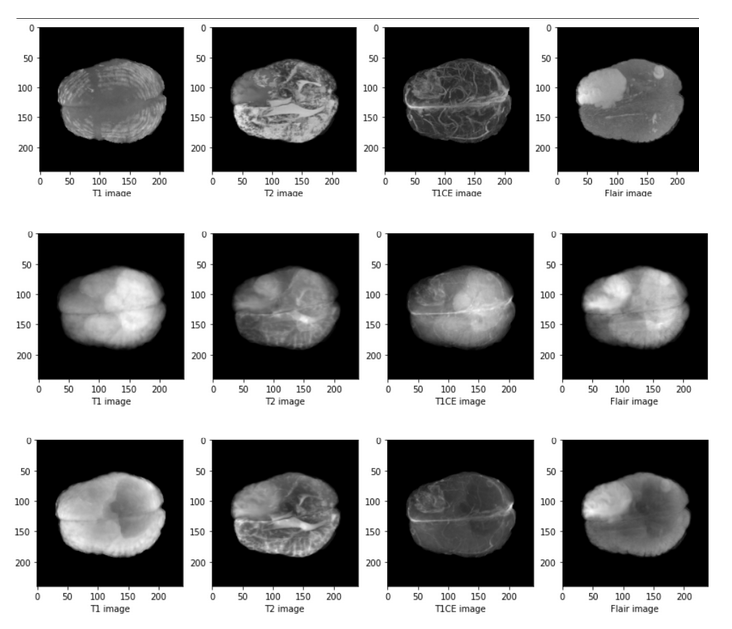
\includegraphics[height=5in]{Methodology/Chapter3Figs/3_projections.png}
    \else
      \includegraphics[bb = 92 86 545 742, height=4.5in]{3_proj}
    \fi
    \caption{\textbf{Row 1} is the Max intensity projection, \textbf{Row 2} is the Mean intensity projection and \textbf{Row 3} is the SD projection}
    \label{3_proj}
  \end{center}
\end{figure}

Classification accuracies was compared with 3 kinds of projections, as well as on 3 different axes (axial, coronal and Saggital). \textbf{EfficientNet B7} was used as a baseline model with \textbf{Focal Loss} as the loss function. Generally, EfficientNet is trained for dimensions of $(x,y,3)$ to incorporate 3-channel RGB, but in this case we used it for predicting 2D images of dimensions $(x,y,1)$.  The results are summarized in the later section \ref{volumetric_results}. 


\section{Cascaded mask-cropped model}\label{cropped_cascaded}
\vspace*{3mm}
One drawback of using the entire tumour image for classification is that it encodes redundant information. The pixels which correspond to the non-tumour tissues can be disposed. Therefore, there is a strong need for a tumour localization strategy that solves this issue. The solution is to train separate classification and segmentation models in a cascaded fashion. 
\vspace*{3mm}

The tumour localization can be done on a pre-determined 2D level or an adaptive 3D level. The 2D approach can have a large bias since the selection of the 2D slice isn't dependent upon the patient scan sample, hence ascertains no effect to the end-to-end pipeline.
\subsection{2D mask-cropped}\label{2D_cropped}
\vspace*{1mm}

\begin{figure}[H]
  \begin{center}
    \leavevmode
    \ifpdf
      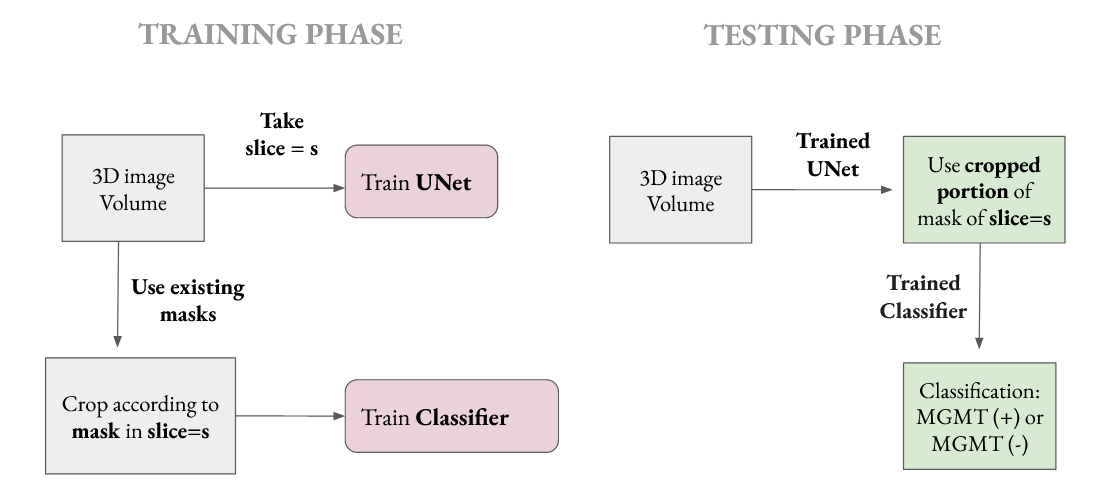
\includegraphics[height=2.5in]{Methodology/Chapter3Figs/2D_cascaded.png}
    \else
      \includegraphics[bb = 92 86 545 742, height=4.5in]{2d_cascaded}
    \fi
    \caption{Training and Testing phases of 2D model}
    \label{2d_cascaded}
  \end{center}
\end{figure}




\begin{algorithm}[H]
\caption{2D cascaded: SEGMENTATION}\label{alg:2D_cascaded_1}
\begin{algorithmic}[1]
\vspace*{4mm}
\Require Slice = s (pre-determined by user)
\For{\texttt{<Each sample in TRAIN set >}}
        \State Extract the slice = s (pre-defined)
        \State Pass that slice to UNet 
        \State Train Unet on all the slices = s 
\EndFor
\State
\For{\texttt{<Each sample in TEST set >}}
    \State Pass the slice = s to UNet
    \State Get the tumour mask
    \State Get the best-bounded-box of the tumour (crop)
    \State Save it in a separate folder
\EndFor

\end{algorithmic}
\end{algorithm}

After we have all the tumour-cropped portions of the train and test set, we move towards the Classifier training. It is to be noted that the cropped regions of the train set are directly obtained from ground-truth masks whereas the cropped regions of the test set are obtained by using the UNet predictions.
\begin{algorithm}[H]
\caption{2D cascaded: CLASSIFICATION}\label{alg:2D_cascaded_2}
\begin{algorithmic}[1]
\vspace*{4mm}
\For{\texttt{<Each sample in TRAIN set >}}
        \State Use ground-truth mask to get cropped image
        \State Pass that cropped slice to Classifier
        \State Train Classifier
\EndFor
\State
\For{\texttt{<Each sample in \textbf{cropped TEST set} >}}
    \State Pass that cropped slice to Classifer
    \State Get methylation prediction probability and output (\textbf{patient level})
\EndFor

\end{algorithmic}
\end{algorithm}
%\vspace*{2mm}

The following images show some examples with the original tumour image, the binary mask and the cropped mask region. 

\begin{figure}[H]
  \begin{center}
    \leavevmode
    \ifpdf
      \includegraphics[height=3.5in]{Methodology/Chapter3Figs/mask_cropped.png}
    \else
      \includegraphics[bb = 92 86 545 742, height=4.5in]{mask_cropped}
    \fi
    \caption{Images with their cropped masked tumours}
    \label{mask_cropped}
  \end{center}
\end{figure}

As classifier, we have used \textbf{ResNet18} and \textbf{EfficientNet B7} with Focal Loss as the classification loss function. The results are summarized in the subsequent section. However, using a pre-determined slice for the pipeline is not desired because it leads to a high bias. Hence, we move to 3D tumour localizations.

\subsection{3D mask cropped}\label{3D_cropped}
\vspace*{4mm}
The 3D tumour localization version takes into account a 3D stacked tumour voxel instead of just a single slice. The central location of the voxel (from the 155 slices) is judged according to the tumour visibility of the slices. The slice with the best tumour visibility is chosen as the middle slice and other slices are taken around it. The tumour visibility is judged by the percentage of '1' labelled pixels in the predicted mask. 

\begin{figure}[H]
  \begin{center}
    \leavevmode
    \ifpdf
      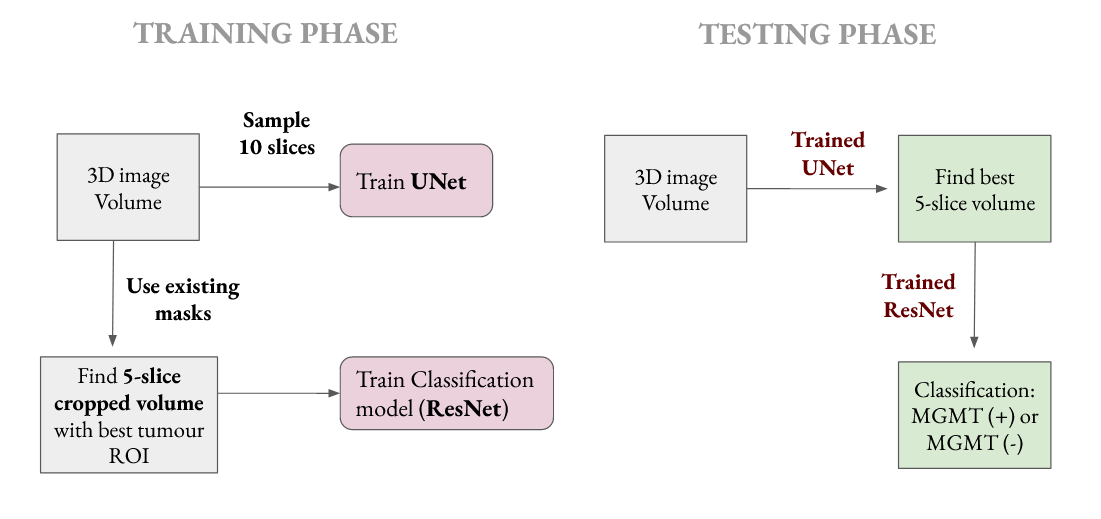
\includegraphics[height=2.7in]{Methodology/Chapter3Figs/cascaded_training_testing.png}
    \else
      \includegraphics[bb = 92 86 545 742, height=4.5in]{3d_cascaded}
    \fi
    \caption{Training and Testing phases of 3D volume model}
    \label{3d_cascaded}
  \end{center}
\end{figure}

After repeated experimentation across all 3 axes (axial, coronal and sagittal) we decided to use a \textbf{5-slice volume} for the 3D localization of the tumour. The middle slice from the 5-sliced stack has the best tumour visible and 2 slices each are chosen from the top and bottom of the chosen best slice.

\begin{algorithm}[H]
\caption{3D cascaded: SEGMENTATION}\label{alg:3D_cascaded_1}
\begin{algorithmic}[1]
\vspace*{2mm}
\For{\texttt{<Each sample in TRAIN set >}}
        \State Sample \textbf{10 slices} (except from top 20\% and bottom 20\% slices)
        \State Train Unet on all the sampled slices 
\EndFor
\For{\texttt{<Each sample in TEST set >}}
    \State Pass \textbf{each slice} to UNet
    \State Get the tumour mask for each slice individually
    \State Find the best slice with most tumour visible, Say $slice = x$
    \State Crop the tumour portions from slices $[x-2, x-1,x,x+1,x+2]$ to get 5-stacked volume
    \State Save 5-stacked volume in a separate folder
\EndFor

\end{algorithmic}
\end{algorithm}
\vspace*{2mm}
\begin{algorithm}[H]
\caption{3D cascaded: CLASSIFICATION}\label{alg:3D_cascaded_2}
\begin{algorithmic}[1]
\vspace*{4mm}
\For{\texttt{<Each sample in TRAIN set >}}
        \State Use ground-truth mask (slice-by-slice) to get $slice=a$ with best tumour visibility
        \State Crop the tumour portions from slices $[a-2, a-1,a,a+1,a+2]$ to get 5-stacked volume
        \State Pass that 3D volume to Classifier
        \State Train Classifier
\EndFor
\State 
\For{\texttt{<Each sample in \textbf{3D cropped TEST set} >}}
    \State Pass that 3D 5-stacked volume to Classifer
    \State Get methylation prediction probability and output (\textbf{patient level})
\EndFor

\end{algorithmic}
\end{algorithm}
\vspace*{4mm}
The benefit of extending the 2D slice version to a 3D volume version is that the pipeline now decides which tumour slice to extract the most information from. A quick iteration across all the given datapoints told us that the tumour location is fairly variable and hence using a pre-set slice is not the best option. Also, training the Unet on 10 samples from each patient scan makes the segmentation more robust for unseen data.
\vspace*{4mm}

The 3D version was tried with various models (across all the 3 axes): \textbf{ResNet18, ResNet34}, the EfficientNet model group (\textbf{EfficientNet B0,EfficientNet B3, EfficientNet B7}. Ensembles of ResNet18 + ResNet34 and ResNet + EfficientNet was also experimented with. The AUCs and accuracies are presented in section \ref{cropped_results}.
\\
\\
\\
\subsection{Ensemble along 3 axes}\label{3-axis-ensemble}
\vspace*{4mm}

The final part of our methodology involved using a 3-axis-ensemble, in which the same patient scan is utilized along the 3 axes (by using 3 separately trained UNet and 3 separately trained Classifiers) and the final predictions are ensembled together to get the final prediction probability. The same 3D MRI scan is sampled along the 3 axis to train the Unet and then used sliced by slice (in testing phase) to get the 5-stack volume which has the best tumour visibility along that particular axis.
\vspace*{4mm}
\begin{figure}[H]
  \begin{center}
    \leavevmode
    \ifpdf
      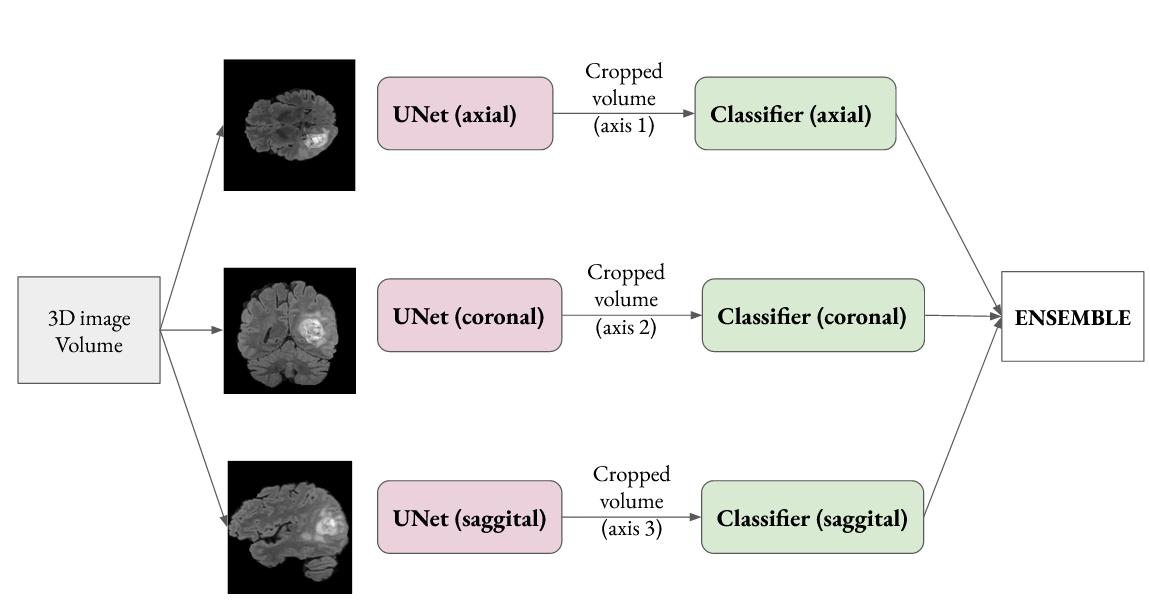
\includegraphics[height=3.2in]{Methodology/Chapter3Figs/3_axis_ensemble.png}
    \else
      \includegraphics[bb = 92 86 545 742, height=4.5in]{3axis}
    \fi
    \caption{3-axis 3D volume classifier ensemble}
    \label{3axis}
  \end{center}
\end{figure}

The classifiers used in each case for each branch was \textbf{ResNet18} and \textbf{ResNet34} since they were lighweight. The number of model parameters becomes three times due to the increased branches of axis 2 and axis 3. The results of the ensemble are shown in section \ref{3_axis_results}.














% ------------------------------------------------------------------------


%%% Local Variables: 
%%% mode: latex
%%% TeX-master: "../thesis"
%%% End: 

% \pagebreak[4]
% \hspace*{1cm}
% \pagebreak[4]
% \hspace*{1cm}
% \pagebreak[4]



\chapter{Results and Discussion}
\ifpdf
    \graphicspath{{Results/Chapter5Figs/PNG/}{Results/Chapter5Figs/PDF/}{Results/Chapter5Figs/}}
\else
    \graphicspath{{Results/Chapter5Figs/EPS/}{Results/Chapter5Figs/}}
\fi

% \begin{eqnarray}
% CIF: \hspace*{5mm}F_0^j(a) &=& \frac{1}{2\pi \iota} \oint_{\gamma} \frac{F_0^j(z)}{z - a} dz
% \end{eqnarray}



                              % first letter Z is for Acronyms 
% \nomenclature[aF]{$F$}{complex function}                                                   % first letter A is for Roman symbols
                                           % first letter G is for Greek Symbols
% \nomenclature[gi]{$\iota$}{unit imaginary number $\sqrt{-1}$}                      % first letter G is for Greek Symbols
% \nomenclature[gg]{$\gamma$}{a simply closed curve on a complex plane}  % first letter G is for Greek Symbols
% \nomenclature[xi]{$\oint_\gamma$}{integration around a curve $\gamma$} % first letter X is for Other Symbols

% first letter R is for superscripts                                                        % first letter S is for subscripts



\hypersetup{ colorlinks=true,
    linkcolor=black,
    filecolor=magenta,      
    urlcolor=blue}


\section{Segmentation results}
\vspace*{3mm}
Before we proceeded to the MTL model inferences, we tested tumour segmentation on the baseline UNet model. Based on a 2D single slice of the MRI scan, we obtained tumour segmentation by categorising each pixel into the labels of \{0,1,2,3\}. As an accuracy metric for segmentation, we used \textbf{IoU (Intersection Over Union)} score. IoU score gives the overlap of the predicted segmentation mask with the actual segmentation mask (This is done classwise. So for 4-class segmentation, 4 IoU scores will be shown). In terms of true-labels and predicted labels (prediction of some label x versus the actual label x), we can come up with another notion of IoU too.

\begin{center}
    $ IoU score$ = $\displaystyle \frac{|A\cap B|}{|A \cup B|}$
    \vspace{3mm}
    \\
    $ IoU score$ = $\displaystyle \frac{TP}{TP + FP + FN}$
\end{center}
~\\
\\
The following table represents the IoU scores obtained solely through UNet when tested across the 4 modalities: T1-weighted, T2-weighted, T1-contrast-enhanced and Flair. 
\vspace{3mm}
\begin{table}[H]
\centering
\begin{tabular}{ c{2cm} c{1.5cm} c{1.5cm} c{1.5cm} c{1.5cm}}
 \hline
 % \multicolumn{5}{c}{\thead{Classwise IoU scores for each modality}} \\
 % [0.8ex]
 % \hline
  \thead{Modality} & \thead{Class 0} & \thead{Class 1} & \thead{Class 2} & \thead{Class 3}\\  [0.8ex]
 \hline
 T1   & 0.982 & 0.209  &0.303 & 0.105  & \\  [0.8ex]
 T2 &   0.983 & 0.223 & 0.371 & 0.089    \\  [0.8ex]
 T1cE & 0.985 & 0.435 & 0.385 & 0.467 &   \\  [0.8ex]
 Flair & 0.991 & 0.067 & 0.472 & 0.113 &  \\  [0.8ex]

 \hline
\end{tabular}
\caption{Classwise IoU scores for each modality}
\label{table:1}
\end{table}

%\vspace{3mm}
%ADD Picture here
\begin{figure}[H]
  \begin{center}
    \leavevmode
    \ifpdf
      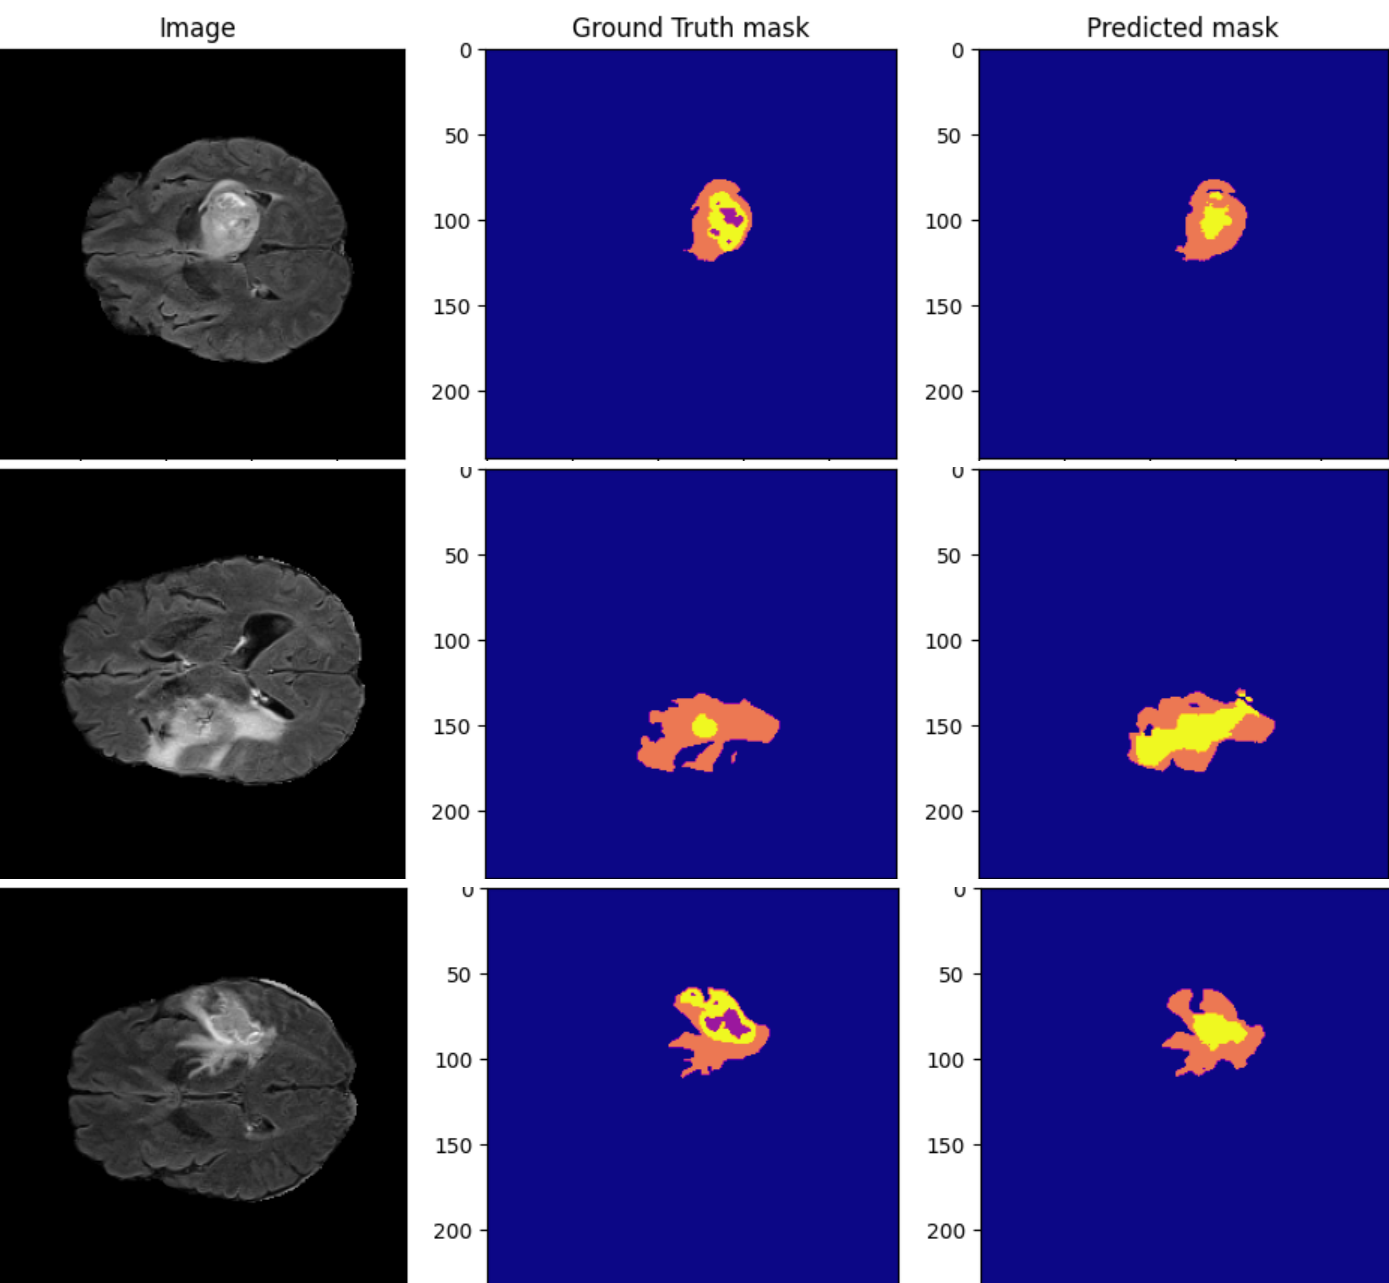
\includegraphics[height=4.2in]{Results/Chapter5Figs/mask_preds.png}
    \else
      \includegraphics[bb = 92 86 545 742, height=4.5in]{mask_pred}
    \fi
    \caption{Tumour mask predictions on test images. Column 1 shows the actual image, followed by the \textbf{Ground truth mask} and the \textbf{Model predictions}}
    \label{mask_pred}
  \end{center}
\end{figure}

The above picture shows some examples of ground-truth segmentation masks and the masks predicted by the UNet model.

\vspace{8mm}
\section{MTL joint segmentation-classification results}\label{MTL_results}
\vspace{3mm}
We experimented with 2 versions of the MTL model (as explained in section \ref{MTL}). One was with just the middle slice = 70 being used as the training set, and another where 10 slices were sampled across all the scans. To get the best possible extent of the nature of model discrimination, we performed the experiment with \textbf{T1-weighted} and \textbf{Flair} images separately. The results are summarized as: 

%3 tables: Flair middle-slice, T1 middle-slice, Flair 10 slices
\vspace{5mm}
\begin{table}[H]
\centering
\begin{tabular}{ c{2cm} c{2cm} c{2cm} c{2cm} c{2cm} }
 \hline
 \multicolumn{5}{c}{\thead{Middle slice : T1-weighted}} \\
 [0.8ex]
 \hline
  \thead{ $\lambda$} &\thead{Mean IoU} & \thead{AUC} & \thead{Accuracy} & \thead{Precision}\\  [0.8ex]
 \hline
  0.1  & 0.735 &0.526 &0.51 & 0.55     &  \\  [0.8ex]
 0.3  &  0.714 & 0.531 & 0.45 & 0.48 & \\  [0.8ex]
0.5  & 0.719 & 0.512 & 0.46 & 0.52  & \\  [0.8ex]
  0.7 & 0.702 & \cellcolor{yellow}\textbf{0.599} & 0.50 & 0.58 &  \\  [0.8ex]
   0.9 & 0.695 & 0.541 & 0.55 & 0.60\\  [0.8ex]

 \hline
\end{tabular}
\caption{Performance of 2D midddle slice MTL (T1)}
\label{table:1}
\end{table}
\vspace{3mm}
\begin{table}[H]
\centering
\begin{tabular}{ c{2cm} c{2cm} c{2cm} c{2cm} c{2cm}  }
 \hline
 \multicolumn{5}{c}{\thead{Middle slice : FLAIR}} \\
 [0.8ex]
 \hline
  \thead{ $\lambda$} & \thead{Mean IoU} & \thead{AUC} & \thead{Accuracy} & \thead{Precision}\\  [0.8ex]
 \hline
 0.1  &  0.868   & 0.542 & 0.58 & 0.58  \\  [0.8ex]
  0.3 & 0.845   & 0.587 & 0.53 & 0.60   \\  [0.8ex]
  0.5 & 0.858 &0.536 &0.52 &  0.56\\  [0.8ex]
  0.7 & 0.851 & 0.534 & 0.51  & 0.56\\  [0.8ex]
  0.9 & 0.793 & 0.441 & 0.45 & 0.50 \\

 \hline
\end{tabular}
\caption{Performance of 2D midddle slice MTL (Flair)}
\label{table:1}
\end{table}
\vspace{3mm}


\begin{table}[H]
\centering
\begin{tabular}{ c{2cm} c{2cm} c{2cm} c{2cm} c{2cm}   }
 \hline
 \multicolumn{5}{c}{\thead{10 sampled slice : Flair}} \\
 [0.8ex]
 \hline
  \thead{ $\lambda$} &\thead{Mean IoU} & \thead{AUC} & \thead{Accuracy} & \thead{Precision}\\  [0.8ex]
 \hline
 0.1 & \cellcolor{yellow}\textbf{0.898}  & 0.4712   & 0.46 & 0.47  \\  [0.8ex]
 0.3 & 0.890   & 0.516 & 0.53 & 0.52   \\  [0.8ex]
 0.5 &  0.882 & 0.497 & 0.51 & 0.50  \\  [0.8ex]
  0.7 & 0.846 & 0.548 & 0.56 & 0.53 \\  [0.8ex]

 \hline
\end{tabular}
\caption{Performance of 2D 10-slice MTL (Flair)}
\label{table:1}
\end{table}
\vspace{3mm}

As can be inferred, the highest AUC \textbf{0.599} is obtained for middle-slice MTL version for the \textbf{T1-weighted} images. The highest mean IoU score over 2 classes segmentation \textbf{0.898} is obtained for the \textbf{Flair} modality by sampling 10 slices. 

\section{Volumetric Projection results}\label{volumetric_results}
\vspace{3mm}
We experimented with 3 kinds of projections: \textbf{Mean, Maximum and Standard Deviation} projections (section \ref{volumetric}). The results of axis 1 (axial direction) for all 3 kinds of projections are depicted below:

\begin{table}[H]
\centering
\begin{tabular}{ c c c c }
 \hline
 \multicolumn{4}{c}{\thead{3 kinds of projection (axial)}} \\
 [0.8ex]
 \hline
  \thead{Projection} & \thead{AUC} & \thead{Accuracy} & \thead{Precision}\\  [0.8ex]
 \hline
 Maximum  & 0.5416  & 0.53 & 0.51  \\  [0.8ex]
 Standard Deviation &  0.5467   & 0.49 & 0.49    \\  [0.8ex]
 Mean &  0.5312 & 0.51 & 0.51   \\  [0.8ex]

 \hline
\end{tabular}
\caption{Projection Performance (axial direction)}
\label{table:1}
\end{table}
\vspace{3mm}

It was observed that the Standard Deviation projection was giving the best results, and so SD projections was tested along all 3 axes: axial, coronal and saggital.
\vspace{3mm}
\begin{table}[H]
\centering
\begin{tabular}{ c c c c }
 \hline
 \multicolumn{4}{c}{\thead{Standard Deviation Projection: 3 axes}} \\
 [0.8ex]
 \hline
  \thead{Axis} & \thead{AUC} & \thead{Accuracy} & \thead{Precision}\\  [0.8ex]
 \hline 
 AXIAL  & \cellcolor{yellow}\textbf{0.5884}    & 0.50 & 0.43 \\  [0.8ex]
 CORONAL &  0.4905  & 0.49 & 0.49   \\  [0.8ex]
 SAGGITAL & 0.5058 & 0.49 & 0.49 \\

 \hline
\end{tabular}
\caption{3 Axis Performance (SD projections)}
\label{table:1}
\end{table}
\vspace{3mm}
\textbf{EfficientNet B7} with \textbf{SD projection (along axial direction)} was the best performance with AUC of \textbf{0.5884}.





\section{Cascaded cropped-mask-results}\label{cropped_results}
\vspace{3mm}
In the cascaded cropped segmentation-classification model (section \ref{cropped_cascaded}), we experimented using 2 strategies: (a) With pre-determined slice number across train and test datasets (section \ref{2D_cropped}) (b) With 5-stack volume by finding the slice with best tumour visibility (section \ref{3D_cropped})
\vspace{3mm}

\textbf{EfficientNet B3, EfficientNet B7} and \textbf{ResNet32} were used for the pre-determined slice version with \textbf{slice = 70} used as the unanimous slice number. The performances are summarized below:
\vspace{3mm}

\begin{table}[H]
\centering
\begin{tabular}{ c c c c }
 \hline
 \multicolumn{4}{c}{\thead{2D slice cascaded model}} \\
 [0.8ex]
 \hline
  \thead{Model} & \thead{AUC} & \thead{Accuracy} & \thead{Precision}\\  [0.8ex]
 \hline
 EfficientNet B3  & 0.6250   & 0.47 & 0.47 \\  [0.8ex]
 EfficientNet B7 &  0.4783   & 0.47 & 0.48    \\  [0.8ex]
 ResNet34 &  \cellcolor{yellow}\textbf{0.6342} & \cellcolor{yellow}\textbf{0.57} & \cellcolor{yellow}\textbf{0.53}  \vspace{3mm}\\ 
 \hline
\end{tabular}
\caption{Results of 2D cascaded model}
\label{table:1}
\end{table}
\vspace{3mm}


We proceeded to the 3D 5-slice stacked volume version of the cascaded model, and the classifiers were changed as: \textbf{EfficientNet B0, EfficientNet B3, EfficientNet B7, ResNet18} and \textbf{ResNet34}. 5 fold cross-validation was utilized with \textbf{Stratified K-folds} strategy to keep the class label ratio similar along all the fold partitions. Henceforth, we used \textbf{5-fold-cross-validation} for each phase. The data mentioned in the tables mention the average AUC/Accuracy with the Standard Deviation obtained across all 5 folds.

\begin{table}[H]
\centering
\begin{tabular}{ c c c c}
 \hline
 \multicolumn{4}{c}{\thead{5-slice 3D cascaded (single classifier)}} \\
 [0.8ex]
 \hline
  \thead{Axis} & \thead{model} & \thead{AUC} & \thead{Accuracy}\\  [0.8ex]
 \hline
 \multirow{5}{4em}{AXIAL}& EffNet B0 & $0.532 \pm 0.038$  & $0.522 \pm 0.046$ & \vspace{3mm}
&EffNet B3 & $0.4942 \pm 0.034$ & $0.506 \pm 0.021$  & \vspace{3mm} 
&EffNet B7 & $0.4455 \pm 0.058$ & $0.5099 \pm 0.017$ & \vspace{3mm}
&ResNet18 & $0.553 \pm 0.062$ & $0.510 \pm 0.047$  & \vspace{3mm}
&ResNet34 & \cellcolor{yellow}\boldmath{$0.641 \pm 0.187$ } & \cellcolor{yellow}\boldmath{$0.620 \pm 0.150$} & 
\hline
\multirow{5}{4em}{CORONAL}& EffNet B0 & $0.546 \pm 0.052$ & $0.493 \pm 0.019$ & \vspace{3mm}
&EffNet B3 & $0.521 \pm 0.044$ & $0.513 \pm 0.018$ & \vspace{3mm} 
&EffNet B7 & $0.475 \pm 0.055$ & $0.511 \pm 0.017$  & \vspace{3mm}
&ResNet18 & $0.640 \pm 0.190$ & $0.608 \pm 0.182$ & \vspace{3mm}
&ResNet34 & $0.586 \pm 0.121$ & $0.574 \pm 0.090$ & 
\hline
\multirow{5}{4em}{SAGGITAL}& EffNet B0 & $0.490 \pm 0.086$ & $0.511 \pm 0.018$ & \vspace{3mm}
&EffNet B3 & $0.505 \pm 0.054 $ & $0.511 \pm 0.017$  & \vspace{3mm} 
&EffNet B7 & $0.509 \pm 0.060$ & $0.488 \pm 0.017$ & \vspace{3mm}
&ResNet18 & $0.582 \pm 0.147$ & $0.576 \pm 0.118$ & \vspace{3mm}
&ResNet34 &  $0.575 \pm 0.183$& $0.551 \pm 0.150$ & 
 \hline
\end{tabular}
\caption{Results of 5-slice 3D cascaded (single model)}
\label{table:1}
\end{table}
\vspace{3mm}

The highest AUC of \boldmath{$0.641 \pm 0.187$} is obtained for \textbf{ResNet34} in the \textbf{axial direction} (as highlighted in the tables). Various kinds of ensembles were also tested with, and in majority of the cases they gave better performances.
\vspace{5mm}
\begin{table}[H]
\centering
\begin{tabular}{ c c c c}
 \hline
 \multicolumn{4}{c}{\thead{5-slice 3D cascaded (ensemble)}} \\
 [0.8ex]
 \hline
  \thead{Axis} & \thead{model} & \thead{AUC} & \thead{Accuracy}\\  [0.8ex]
 \hline
 \multirow{3}{4em}{AXIAL}& ResNet18 + ResNet34 & \cellcolor{yellow}\boldmath{$0.736 \pm 0.160$} & \cellcolor{yellow}\boldmath{$ 0.662 \pm 0.148$} & \vspace{3mm}
&ResNet18 + EffNet B3 & $0.692 \pm 0.169$  & $0.653 \pm 0.140$ & \vspace{3mm} 
&ResNet34 + EffNet B3 & $0.713 \pm 0.160$ & $0.662 \pm 0.148$ & 
\hline
\multirow{3}{4em}{CORONAL}& ResNet18 + ResNet34 & \cellcolor{yellow}\boldmath{$0.721 \pm 0.174$} & \cellcolor{yellow}\boldmath{$ 0.693 \pm 0.140$} & \vspace{3mm}
&ResNet18 + EffNet B3 & $0.680 \pm 0.199$ & $0.637 \pm 0.172$ & \vspace{3mm} 
&ResNet34 + EffNet B3 & $0.637 \pm 0.177$ & $0.608 \pm 0.136$ & 
\hline
\multirow{3}{4em}{SAGGITAL}& ResNet18 + ResNet34 & $0.707 \pm 0.202$ & $0.684 \pm 0.154$ & \vspace{3mm}
&ResNet18 + EffNet B3 & $0.629 \pm 0.189$ & $0.609 \pm 0.135$ & \vspace{3mm} 
&ResNet34 + EffNet B3 & $0.715 \pm 0.146$ & $0.671 \pm 0.104$ & 
 \hline
\end{tabular}
\caption{Results of 5-slice 3D cascaded (ENSEMBLE)}
\label{table:1}
\end{table}
\vspace{3mm}
For ensembles, the highest AUC \boldmath{$0.736 \pm 0.160$} is obtained for the \textbf{ResNet18 and ResNet34 ensemble} in the \textbf{axial direction} and the highest Accuracy \bolmath{$0.693 \pm 0.140$} is obtained for the same emsemble in the \textbf{coronal direction} (as highlighted in the tables).


\section{3-axis Ensemble Results}\label{3_axis_results}
\vspace{3mm}
The 3-axis-ensemble (section \ref{3-axis-ensemble}) uses the same MRI scan to sample slices across 3 different axis directions, and then trains separte UNet and classifiers for each direction.
\vspace{4mm}

\begin{table}[H]
\centering
\begin{tabular}{ c c c c}
 \hline
 \multicolumn{3}{c}{\thead{3-axis ensemble}} \\
 [0.8ex]
 \hline
  \thead{Model} & \thead{AUC} & \thead{Accuracy} \\  [0.8ex]
 \hline
 ResNet18  &  $0.711 \pm 0.198$   & $0.665 \pm 0.171$  \\  [0.8ex]
 ResNet34 &  \cellcolor{yellow}\boldmath{$0.721 \pm 0.231$}  & \cellcolor{yellow}\boldmath{$0.700 \pm 0.205$ }  & \vspace{3mm}\\ 
 \hline
\end{tabular}
\caption{Results of 3-axis Ensemble}
\label{table:1}
\end{table}
\vspace{3mm}


As a conclusion across all models tested, we were able to attain the highest AUC \textbf{0.736} in \textbf{ResNet18 + ResNet34 ensemble} in the axial directional case. This surpasses the current Kaggle leaderboard AUC of abc.

\vspace{5mm}
AUC in the experimentation refers to Area under curve, which has been explained in Appendix A (\ref{AUC}). AUC is calculated as the Area Under the $Sensitivity$(TPR)-$(1-Specificity)$(FPR) Curve. True Positive refers to the samples which were classified as '1' (methylated) and it was a correct classification, while FP refers to a '1' classification which was False (truth was unmethylated).
\\
\begin{center}
    $Accuracy$ = $\displaystyle\frac{TP+TN}{TP+TN+FP+FN}$
\\\vspace{2mm}
$Precision $= $\displaystyle\frac{TP}{TP+FP}$
\\\vspace{2mm}
$Recall $=$ \displaystyle\frac{TP}{TP+FN}$
\\\vspace{4mm}
\end{center}





% \cite{texbook}

% \subsection{sub first paragraph}
% ... and some more ...



% above code has been macro-fied in Classes/MacroFile.tex file
%\InsertFig{\IncludeGraphicsH{aflow}{6in}{92 86 545 742}}{Airfoil Picture}{FigAir}

% So as we have now labelled it we can reference it, like so (\ref{FigKaggleLeaderboard}) and it
% is on Page \pageref{FigKaggleLeaderboard}. And as we can see, it is a very nice picture and we
% can talk about it all we want and when we are tired we can move on to the next
% chapter ...

\ifpdf
  \pdfbookmark[2]{bookmark text is here}{And this is what I want bookmarked}
\fi
% ------------------------------------------------------------------------


%%% Local Variables: 
%%% mode: latex
%%% TeX-master: "../thesis"
%%% End: 





\backmatter
\def\baselinestretch{1}
\chapter{Conclusion}
\ifpdf
    \graphicspath{{Conclusions/ConclusionsFigs/PNG/}{Conclusions/ConclusionsFigs/PDF/}{Conclusions/ConclusionsFigs/}}
\else
    \graphicspath{{Conclusions/ConclusionsFigs/EPS/}{Conclusions/ConclusionsFigs/}}
\fi

\def\baselinestretch{1.66}

The proposed end-to-end tumour segmentation pipeline can be used assistively to aid medical practioners in detecting and assessing the methylation of glioblastoma, in order to increase the chemotherapy benefits of TMZ. Since our model is sufficiently lightweight, it can save time in processing a large quantity of MRI scans. As limitations to the proposed approach, it should be noted that because the dataset size was quite small, an experimental bias could have been incurred. Further research could be done to build more nuanced models by combining the MRI modalities and give more emphasis on predicting the methylation status through a countinuos value (across all the gene markers) rather than limiting to a simple binary classification.

%%% ----------------------------------------------------------------------

% ------------------------------------------------------------------------

%%% Local Variables: 
%%% mode: latex
%%% TeX-master: "../thesis"
%%% End: 
% book mode only
\appendix
\chapter{Appendix A : Area Under Curve (AUC)}\label{AUC}

The ROC: Receiver Operating characteristic curve analyses discriminatory capability of any binary classifier in machine learning. Area Under the ROC Curve (AUC) has been widely used to judge the performance of classification models. 
\vspace{3mm}

Normally, while using a Softmax layer in the last layer of any binary classification model, we get the output as the vector [x,y] where x and y represent the classification probability of the sample belonging to class 0 or class 1 respectively. Based on a threshold value (given), the activation function decides which class to assign. Thereafter when we calculate the Accuracy, Precision, Recall we are generally counting how many samples were classified correctly and how many were classified incorrectly. The count of assigned samples depends upon the threshold value assigned during classification.
\vspace{3mm}
\begin{center}
    Sensitivity = Recall = $\displaystyle\frac{TP}{TP+FN}$
    \\
Specificity = $\displaystyle\frac{TN}{FP+TN}$ \\
\end{center}

AUC is calculated as the Area Under the $Sensitivity$(TPR) versus the $(1-Specificity)$(FPR) Curve. With an increasing sets of thresholds (0\% to 100\%) it calculates the TPR and FPR in each case, and plots a point in the AUC curve. When all the thresholds have been plotted, it calculates the integral area under the curve. AUC 0 signifies a model with 100\% wrong predictions while AUC 1 means a model with 100\% correct predictions.



% ------------------------------------------------------------------------

%%% Local Variables: 
%%% mode: latex
%%% TeX-master: "../thesis"
%%% End: 


\bibliographystyle{plainnat}
%\bibliographystyle{Classes/IITRPRbiblio}
\renewcommand{\bibname}{References} % changes default name Bibliography to References
\bibliography{References/references} % References file

\end{document}
